\documentclass[tikz, border=10pt]{standalone}
\usepackage{tikz}
\usetikzlibrary{angles, quotes, calc}

\begin{document}
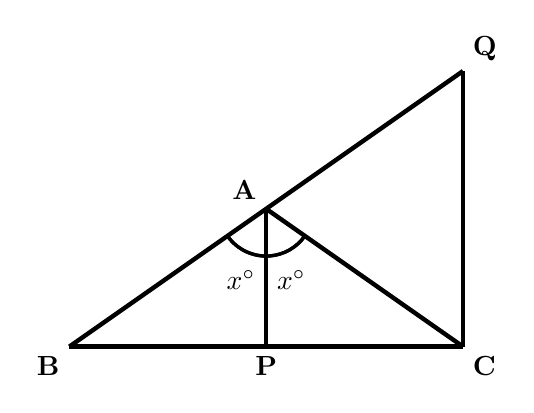
\begin{tikzpicture}

% Define points
\coordinate (B) at (0, 0);
\coordinate (C) at (5, 0);
\coordinate (Q) at (5, 3.5);

% A is on line BQ
\coordinate (A) at ($(B)!0.5!(Q)$);

% P is on BC (below A approximately)
\coordinate (P) at (2.5, 0);

% Draw base BC
\draw[ultra thick] (B) -- (C);

% Draw line from B through A to Q
\draw[ultra thick] (B) -- (Q);

% Draw line AC
\draw[ultra thick] (A) -- (C);

% Draw line CQ
\draw[ultra thick] (C) -- (Q);

% Draw line AP
\draw[ultra thick] (A) -- (P);

% Draw angle arcs at P
% Angle BPA (left side)
\pic[draw, very thick, left, angle radius=0.6cm, angle eccentricity=1.5, "$x^{\circ}$"] {angle=B--A--C};

\pic[draw, very thick, right, angle radius=0.6cm, angle eccentricity=1.5, "$x^{\circ}$"] {angle=B--A--C};

% Labels
\node[below left] at (B) {\textbf{B}};
\node[below right] at (C) {\textbf{C}};
\node[above right] at (Q) {\textbf{Q}};
\node[below] at (P) {\textbf{P}};
\node[above left] at (A) {\textbf{A}};

\end{tikzpicture}
\end{document}